% Options for packages loaded elsewhere
\PassOptionsToPackage{unicode}{hyperref}
\PassOptionsToPackage{hyphens}{url}
\PassOptionsToPackage{dvipsnames,svgnames,x11names}{xcolor}
%
\documentclass[
  super,
  preprint,
  3p]{elsarticle}

\usepackage{amsmath,amssymb}
\usepackage{setspace}
\usepackage{iftex}
\ifPDFTeX
  \usepackage[T1]{fontenc}
  \usepackage[utf8]{inputenc}
  \usepackage{textcomp} % provide euro and other symbols
\else % if luatex or xetex
  \usepackage{unicode-math}
  \defaultfontfeatures{Scale=MatchLowercase}
  \defaultfontfeatures[\rmfamily]{Ligatures=TeX,Scale=1}
\fi
\usepackage{lmodern}
\ifPDFTeX\else  
    % xetex/luatex font selection
\fi
% Use upquote if available, for straight quotes in verbatim environments
\IfFileExists{upquote.sty}{\usepackage{upquote}}{}
\IfFileExists{microtype.sty}{% use microtype if available
  \usepackage[]{microtype}
  \UseMicrotypeSet[protrusion]{basicmath} % disable protrusion for tt fonts
}{}
\makeatletter
\@ifundefined{KOMAClassName}{% if non-KOMA class
  \IfFileExists{parskip.sty}{%
    \usepackage{parskip}
  }{% else
    \setlength{\parindent}{0pt}
    \setlength{\parskip}{6pt plus 2pt minus 1pt}}
}{% if KOMA class
  \KOMAoptions{parskip=half}}
\makeatother
\usepackage{xcolor}
\setlength{\emergencystretch}{3em} % prevent overfull lines
\setcounter{secnumdepth}{5}
% Make \paragraph and \subparagraph free-standing
\ifx\paragraph\undefined\else
  \let\oldparagraph\paragraph
  \renewcommand{\paragraph}[1]{\oldparagraph{#1}\mbox{}}
\fi
\ifx\subparagraph\undefined\else
  \let\oldsubparagraph\subparagraph
  \renewcommand{\subparagraph}[1]{\oldsubparagraph{#1}\mbox{}}
\fi


\providecommand{\tightlist}{%
  \setlength{\itemsep}{0pt}\setlength{\parskip}{0pt}}\usepackage{longtable,booktabs,array}
\usepackage{calc} % for calculating minipage widths
% Correct order of tables after \paragraph or \subparagraph
\usepackage{etoolbox}
\makeatletter
\patchcmd\longtable{\par}{\if@noskipsec\mbox{}\fi\par}{}{}
\makeatother
% Allow footnotes in longtable head/foot
\IfFileExists{footnotehyper.sty}{\usepackage{footnotehyper}}{\usepackage{footnote}}
\makesavenoteenv{longtable}
\usepackage{graphicx}
\makeatletter
\def\maxwidth{\ifdim\Gin@nat@width>\linewidth\linewidth\else\Gin@nat@width\fi}
\def\maxheight{\ifdim\Gin@nat@height>\textheight\textheight\else\Gin@nat@height\fi}
\makeatother
% Scale images if necessary, so that they will not overflow the page
% margins by default, and it is still possible to overwrite the defaults
% using explicit options in \includegraphics[width, height, ...]{}
\setkeys{Gin}{width=\maxwidth,height=\maxheight,keepaspectratio}
% Set default figure placement to htbp
\makeatletter
\def\fps@figure{htbp}
\makeatother

\usepackage{booktabs}
\usepackage{longtable}
\usepackage{array}
\usepackage{multirow}
\usepackage{wrapfig}
\usepackage{float}
\usepackage{colortbl}
\usepackage{pdflscape}
\usepackage{tabu}
\usepackage{threeparttable}
\usepackage{threeparttablex}
\usepackage[normalem]{ulem}
\usepackage{makecell}
\usepackage{xcolor}
\makeatletter
\@ifpackageloaded{caption}{}{\usepackage{caption}}
\AtBeginDocument{%
\ifdefined\contentsname
  \renewcommand*\contentsname{Table of contents}
\else
  \newcommand\contentsname{Table of contents}
\fi
\ifdefined\listfigurename
  \renewcommand*\listfigurename{List of Figures}
\else
  \newcommand\listfigurename{List of Figures}
\fi
\ifdefined\listtablename
  \renewcommand*\listtablename{List of Tables}
\else
  \newcommand\listtablename{List of Tables}
\fi
\ifdefined\figurename
  \renewcommand*\figurename{Figure}
\else
  \newcommand\figurename{Figure}
\fi
\ifdefined\tablename
  \renewcommand*\tablename{Table}
\else
  \newcommand\tablename{Table}
\fi
}
\@ifpackageloaded{float}{}{\usepackage{float}}
\floatstyle{ruled}
\@ifundefined{c@chapter}{\newfloat{codelisting}{h}{lop}}{\newfloat{codelisting}{h}{lop}[chapter]}
\floatname{codelisting}{Listing}
\newcommand*\listoflistings{\listof{codelisting}{List of Listings}}
\makeatother
\makeatletter
\makeatother
\makeatletter
\@ifpackageloaded{caption}{}{\usepackage{caption}}
\@ifpackageloaded{subcaption}{}{\usepackage{subcaption}}
\makeatother
\journal{European Transport Research Review}
\ifLuaTeX
  \usepackage{selnolig}  % disable illegal ligatures
\fi
\usepackage[]{natbib}
\bibliographystyle{elsarticle-num}
\usepackage{bookmark}

\IfFileExists{xurl.sty}{\usepackage{xurl}}{} % add URL line breaks if available
\urlstyle{same} % disable monospaced font for URLs
\hypersetup{
  pdftitle={Cycle Route Uptake and Scenario Estimation (CRUSE): an approach for developing strategic cycle network planning tools},
  pdfauthor={Robin Lovelace; Joey Talbot; Eugeni Vidal-Tortosa; Hussein Mahfouz; Elaine Brick; Peter Wright; Gary O'Toole; Dan Brennan; Suzanne Meade},
  pdfkeywords={Cycling, Open-source, Road Safety, Active
Travel, Transport Planning, Collaborative Planning},
  colorlinks=true,
  linkcolor={blue},
  filecolor={Maroon},
  citecolor={Blue},
  urlcolor={Blue},
  pdfcreator={LaTeX via pandoc}}

\setlength{\parindent}{6pt}
\begin{document}

\begin{frontmatter}
\title{Cycle Route Uptake and Scenario Estimation (CRUSE): an approach
for developing strategic cycle network planning tools}
\author[1]{Robin Lovelace%
\corref{cor1}%
}
 \ead{r.lovelace@leeds.ac.uk} 
\author[1]{Joey Talbot%
%
}

\author[1]{Eugeni Vidal-Tortosa%
%
}

\author[1]{Hussein Mahfouz%
%
}

\author[2]{Elaine Brick%
%
}

\author[3]{Peter Wright%
%
}

\author[2]{Gary O'Toole%
%
}

\author[4]{Dan Brennan%
%
}

\author[4]{Suzanne Meade%
%
}


\affiliation[1]{organization={University of
Leeds},addressline={Institute for Transport Studies, Leeds, LS2 9JT,
United Kingdom},postcodesep={}}
\affiliation[2]{organization={AECOM},addressline={Unit 6, Galway
Technology Park, Parkmore, Galway, Ireland},postcodesep={}}
\affiliation[3]{organization={AECOM},addressline={Winslade House,
Winslade Park, Manor Drive, Clyst St Mary, Exeter, EX5 1FY,
UK},postcodesep={}}
\affiliation[4]{organization={Transport Infrastructure
Ireland},addressline={Parkgate Business Centre, Parkgate Street, Dublin
8, D08 DK10, Ireland},postcodesep={}}

\cortext[cor1]{Corresponding author}









        
\begin{abstract}
This paper describes an approach for developing strategic cycle network
planning tools. Based on our experience developing and deploying the
Cycle Route Uptake and Scenario Estimation (CRUSE) Tool for Ireland, we
outline the underlying methods, including disaggregation of
origin-destination data, incorporation of additional trip purposes,
routing, scenario generation, and development of an intuitive user
interface that has been tested and used by practitioners. Commissioned
and used by Transport Infrastructure Ireland, CRUSE provides estimates
of current and potential future cycling levels under `snapshot'
scenarios to inform investment decisions. The publicly available results
at https://cruse.bike/ enable planners, engineers, and other
stakeholders to make more evidence-based decisions. CRUSE goes beyond
previous work by: modeling networks at high spatial resolution;
simulating multiple trip purposes (social, shopping, personal utility,
recreational, and cycle touring) in addition to using official
origin-destination data; and providing estimates of `quietness' (a proxy
for cyclist comfort and route preference) at the route segment level.
Three network types --- `Fastest', `Balanced', and `Quietest' --- help
plan both arterial and residential cycle networks. Workshops and
unstructured interviews with stakeholders show that the tool is already
being used in practice to inform urban, inter-urban, and rural network
planning. The approach is flexible and open-source, allowing the
underlying ideas and code to be adapted, supporting effective cycling
policies and interventions internationally.
\end{abstract}





\begin{keyword}
    Cycling \sep Open-source \sep Road Safety \sep Active
Travel \sep Transport Planning \sep 
    Collaborative Planning
\end{keyword}
\end{frontmatter}
    
\setstretch{2}
\newpage{}

\section{Introduction}\label{introduction}

\subsection{Background}\label{background}

Transport systems dominated by heavy and powerful private cars are
inefficient, dangerous, and unhealthy. Cars are a major and growing
source of greenhouse gas (GHG) emissions \citep{winkler2023}, a leading
cause of premature death and injury due to road traffic collisions
\citep{globals2018}, and a cause of disease due to physical inactivity
and air, noise and microplastic pollution \citep{mattsson2023}
\citep{welch2023} \citep{cavallaro2024}. Transport is responsible for
23\% of GHG emissions, 70\% of which are from road transport, with
passenger cars accounting for nearly half of transport emissions (around
10\% of global emissions) \citep{jaramillo2022}. The transport system
encourages, enables and in some cases enforces unsustainable lifestyles.
Services that are only accessible by car lock-in car dependency
\citep{gray2001, shergold2012, motte-baumvol2010}.

Growing evidence of the negative impacts of car-dependent transport
systems has led governments in many countries to set targets and take
actions. In the context of climate, road safety and physicial inactivity
crises, policies to improve transport systems can be classified
according to the `Avoid-Shift-Improve' (ASI) framework
\citep{jaramillo2022}. The ASI framework highlights the importance of
demand reduction (\emph{avoid}ing unnecessary trips), in addition to
mode \emph{shift} to sustainable modes and \emph{improvement} of
existing energy converters, in that order.

Building cycle networks represents a relatively `quick win' within the
context of decarbonization \citep{brand2020} and sustainable mobility
\citep{burns2013}. Although cycling uptake appears on the surface to
only relate to the `shift' part of the ASI framework, closer
consideration of the knock-on impacts of cycling uptake shows that it
can also help avoid unnecessary trips \citep{nello-deakin2020}.
Furthermore, highly efficient ebikes --- which are seeing rapid uptake
--- outperform electric cars, which are too heavy and expensive, for the
majority of trips. Over-reliance on electric cars could slow the
transition away from car dependency and inadvertently enable ``high
travel lock-in'' \citep{anable2019}. At the European level, the European
Union has a target of reducing GHG emissions by 55\% by 2030, compared
to 1990 levels, and to achieve `net-zero' by 2050 \citep{rosenow2022}.
Climate change mitigation is a major motivation for cycle network plans
\citep{scappini2022}.

Another motivation for cycle network planning at the European level is
the Road Infrastructure Safety Management (RISM) directive (2008/96/EC),
which requires member states to implement a road safety management
system (RSMS) for all public roads. Specifically, ``Member States shall
ensure that the ranking of high accident concentration sections and the
network safety ranking are carried out'' \citep{directiv2008}. Given
that `safety' in this context is usefully quantified as the number of
people killed or seriously injured (KSI) per distance traveled, the
directive requires estimation of distance traveled by mode, down to the
road link level. For active modes, about which there is a paucity of
data compared with motorized modes, this is a major challenge. Better
data to inform road safety policies and interventions is a motivation
for better estimates of `baseline' levels of physical activity at high
geographic resolutions \citep{tait2023}.

National governments are increasingly acting on the evidence. In
Ireland, the Road Safety Authority (RSA) has set the target of halving
the number of road traffic deaths and serious injuries by 2030
\citep{national2021}. Doing so while simultaneously enabling rapid
uptake of active modes will require key travel corridors to be
identified and `cycle proofed'. Cycling in Ireland represents only 3\%
of total modal share as of the 2016 Census, but accounts for 20\% of
serious injuries and 7\% of all fatalities. Poor perception of safety
has been found to represent the most important barrier to increased
cycling in Ireland\citep{brick2018}, and the need to improve road safety
drives the development of national cycling policy and infrastructure
plans. The main frameworks underpinning these efforts are the Climate
Action Plan \citep{climate2022a}, the National Development Plan, and the
National Roads 2040 strategy \citep{national2023}.

At the regional level within Ireland, the recently published Greater
Dublin Area Transport Strategy \citep{greater} reveals the high support
for and capability for cycling: ``nearly a quarter of adults cycle at
least once a week in the Dublin Metropolitan Area'' with cycling in the
Dublin area taking up to 60,000 cars off the road today. Extrapolating
this on a per population basis across Ireland, with around 40\% of the
population living in Dublin, suggests that around 150,000 cars could be
removed nationwide just by achieving Dublin levels of cycling in all
counties (notwithstanding existing cycling trips and differences in trip
distances). Seven in ten trips in Ireland are by car \citep{national}.
Cycling has the potential to replace a large proportion of these trips:
``A high priority must also be given to cyclists, because trips by this
mode have the potential to replace trips by private car, most
specifically for short to medium distance trips, but increasingly for
longer trips as ebikes extend the range of this mode'' \citep{greater}.

Further evidence of the importance of cycling in Ireland is provided by
the National Strategic Objective (NSO) from the National Development
Plan, which allocates €8.6 billion to sustainable transport
infrastructure including public transport and active travel
interventions. Cycle infrastructure will be developed in synchrony with
the BusConnects project, an entire redesign of the bus network in Dublin
and Cork. It was in this context that Transport Infrastructure Ireland
(TII) commissioned the research reported in this paper, which led to the
Cycle Route Uptake and Scenario Estimation (CRUSE) Tool for Ireland.
Building on previous work, including the Propensity to Cycle Tool (PCT)
for England and Wales, the CRUSE Tool was developed to provide evidence
on current cycling levels and future cycling potential nationwide across
Ireland.

Stakeholder consultation by TII emphasized the need for a strong,
national, systematic but locally-specific evidence base on cycle
networks in both urban and rural Ireland. The evidence base had to scale
nationally to support strategic alignment with national, regional and
local policies, but also be useful for local network planning.

\subsection{Aim and content}\label{aim-and-content}

This paper describes an approach to strategic cycle network planning
tool development that is open, scalable, and evidence-based. We label
the approach Cycle Route Uptake and Scenario Estimation (CRUSE) and
present a case study of its application in Ireland, the results of which
are publicly available at \href{https://cruse.bike/}{cruse.bike}.

In Section~\ref{sec-tools}, we review existing current tools for
estimating cycling potential. In Section~\ref{sec-methods}, we outline
the methods used to generate the evidence presented in the CRUSE Tool.
In Section~\ref{sec-results}, we present the results of the CRUSE Tool,
including estimates of current cycling levels and future cycling
potential at the national, regional and local levels. In
Section~\ref{sec-discussion}, we discuss limitations and possible future
improvements to the approach, and the implications of the results for
Ireland before making concluding remarks in
Section~\ref{sec-conclusions}.

\section{Tools for estimating cycling potential}\label{sec-tools}

Tools for estimating geographical distribution of cycling potential have
advanced substantially in recent years. Developed by researchers and
developers in academic, public and private sectors, they have evolved
from simple area-based static models tailored to specific regions to
more complex and (in some cases) more generalizable tools. These tools
can be considered as a specific application of the concept of planning
support systems (PSS) , which are designed to help planners and
decision-makers to make more informed decisions \citep{geertman2009}.
Outputs include maps with results available at several levels of
analysis with levels of availability ranging from being only available
to researchers and in static maps to open access mapping systems
available to the public.

Previous studies have applied the concept of PSS to specific modes,
including walking \citep{bencekri2024}, public transport
\citep{barmentlo2012} and cycling \citep{bencekri2023}. While such prior
work provides insight into the potential for approaches to transport
planning that are both data-driven and participatory, the focus of this
paper is on tools that focus attention on the \emph{geographic
distribution} of cycling potential and which answer the question ``where
to build''. Not all papers reviewed in this section classify themselves
as, or even mention, PSS, but all of them can be considered as PSS. This
paper is informed by the thinking underlying PSS, including the idea
that the resulting tools are more effective if they are modular and can
inter-link with other tools and processes in the planning process: PSS
can be conceived as a ``toolbox with separate instruments that can work
and talk to each other effectively (as in the open systems concept) and
that will be selectively applied in varying configurations to support a
particular phase in the planning process'' \citep{geertman2002}. We
share this conception of PSS, emphasizing the benefits of a focus on a
particular mode (cycling) and a particular phase in the planning process
(strategic network development).

Some of the most relevant existing tools are summarised below and
presented in Table~\ref{tbl-tools}.

\begin{longtable}[t]{>{\raggedright\arraybackslash}p{13em}>{\raggedright\arraybackslash}p{15em}>{\raggedright\arraybackslash}p{12em}>{\raggedright\arraybackslash}p{5em}}

\caption{\label{tbl-tools}Summary of existing tools for estimating
cycling potential.}

\tabularnewline

\\
\toprule
Approach & Coverage and input data & Outputs and availability & License\\
\midrule
\cellcolor{gray!10}{Bicycle share model, Parkin et al. (2007)} & \cellcolor{gray!10}{England and Wales, Journeys to work OD census data, at the small-area (wards) level} & \cellcolor{gray!10}{Static tables in academic paper} & \cellcolor{gray!10}{Proprietary}\\
Analysis of  Cycling Potential (ACP), Transport for London (2010, 2016) & London, London Travel Demand Survey & Static tables, graphs, and heatmaps, not publicly available & Proprietary\\
\cellcolor{gray!10}{Prioritization index, Larsen et al. (2013)} & \cellcolor{gray!10}{Montreal, Survey, Road safety, and OD data} & \cellcolor{gray!10}{Map-based heatmap, not publicly available} & \cellcolor{gray!10}{Proprietary}\\
Usage intensity index, Zhang et al. (2014) & Belo Horizonte, Survey, census, and OD data & Static tables and maps, not publicly available & Proprietary\\
\cellcolor{gray!10}{The Cycling Potential Tool (CPT), Phillips and Range (2017)} & \cellcolor{gray!10}{Scotland, Environmental and socioeconomic data, at the small area (output areas) level} & \cellcolor{gray!10}{Maps showing cycling potential in each area} & \cellcolor{gray!10}{Proprietary}\\
\addlinespace
Propensity to Cycle Tool (PCT), Lovelace et al. (2017) & England and Wales, Journeys to work and school OD census data, at the small area (LSOA) level & Online maps, graphs, tables, publicly available at www.pct.bike & Open source\\
\cellcolor{gray!10}{The    Gross Potential for Cycling tool (CPC), Silva et al. (2021 and 2022)} & \cellcolor{gray!10}{21 Portuguese cities, Land use and socio-demographic data, at the small area (census tract) level} & \cellcolor{gray!10}{Static maps showing cycling potential in different areas} & \cellcolor{gray!10}{NA}\\
\bottomrule

\end{longtable}

Area-based approaches were developed before network-based tools, such as
a 2007 regression-based model to estimate the percentage of cycling
trips to work in England and Wales based on socioeconomic,
transportation, and physical factors at the small area (wards) level in
2007 \citep{parkin_estimation_2007}. They found that areas with a higher
percentage of females, non-whites, car ownership, lower socioeconomic
classes, income, distance to work, population density, poor highway
conditions, hills, rainfall, and fewer off-road bicycle routes tended to
have a lower proportion of cycling to work. The approach also generated
``forecasts for potential levels of bicycle use'' with with increases in
off-road routes, improvements of highway and, conversely, increases in
car ownership and distance to work leading to decreases in cycling to
work.

Three years later, Transport for London created the Analysis of Cycling
Potential (ACP) tool based on a mode choice model that assesses the
likelihood of trips being cycled, with data from the TfL London Travel
Demand Survey as its primary input. The tool generates tables, graphs,
and heatmaps showing the potential for cycling for different trips
purposes in London to guide local cycling initiatives, such as where new
hire `docking stations' should go. The tool does not use
origin-destination data and cannot estimate cycling potential on
specific routes \citep{transport_for_london_analysis_2010}.

Other tools that generate areal data to prioritize investment include a
study that generated a `prioritization index' for Montreal, Canada
\citep{larsen_build_2013}, a `usage intensity index' based on stated
preferences in Belo Horizonte, Brazil, and a Cycling Potential Tool
(CPT) for Scotland \citep{phillips_development_2017}. The CPT is
composed of the base environmental module --- based on eight weighted
factors (population density, hilliness, physical barriers, access to
services, existing cycling mode share, distance to work and school, and
road speed) --- and the quality of service module, which evaluates each
area of interest based on eight factors (surface condition, adjacent
cyclists, comfort factor, conflict, distance between junctions, slope,
access to services, and origin/destination).

A more recent areal-based approach is the designed the Gross Potential
for Cycling (GPC) tool to prioritize areas for cycling infrastructure
and other cycling measures \citep{silva_gross_2021}. The GPC uses two
sets of indicators: population-based indicators (age, potential demand
density, employment density and motorization rate) and area-based
indicators (accessibility, education, public transport, connectivity,
land use mix and relative performance). These indicators are calculated
considering topography, road hierarchy, and average congestion and
presented on a scale from 5 to 10. They are then combined into an
overall score, weighted by their impact on cycling according to the
literature. The ranking of areas by the GPC are
\href{https://boost.up.pt/en/ferramentas/gpc}{publicly available} and
its practical value has been assessed through workshops
\citep{silva_revealing_2022}.

Route-based tools emerged with increasing availability of
origin-destination data, routing engines that can assign trips to
networks, and improvements in computer hardware and software needed to
generate route networks. A prominent example is the the Propensity to
Cycle Tool (PCT), first developed to estimate current and future levels
of cycling at desire line, zone, route, and route network levels for
case study cities \citep{lovelace_mapping_2016}. The approach was
scaled-up to estimate estimate the potential benefits of uptake at zone
and desire line levels nationally, and launched as a publicly available
web application in 2017 \citep{lovelace2017}. Extensions of the PCT
approach have included estimation of benefits at the individual level
\citep{woodcock2018}, addition of travel to school network
\citep{goodman2019}, and improved modeling of impacts on health,
environmental and distributional outcomes \citep{woodcock2021}.
Initially developed just for England, the PCT was extended to cover all
of Wales (for commuter data only) in 2018.

The PCT approach has been applied in other countries, including Ireland
(the topic of this paper), Scotland, and Portugal. In Portugal the
`biclaR' project, based on methods underlying the PCT, has been
developed and deployed for the Lisbon metro region. The resulting
evidence is available in an interactive web application hosted at
\href{https://biclar.tmlmobilidade.pt}{biclar.tmlmobilidade.pt}
\citep{felix2023}. biclaR includes estimates of impacts, using the World
Health Organisation (WHO) `HEAT for Cycling' tool and an `intermodality'
scenario that combines cycling with currently available public transit
options based on General Transit Feed Specification (GTFS) data.

The approach presented in this paper seeks to overcome three limitations
of previous tools to estimate cycling potential: 1) low resolution of
data, with routes starting and ending in administrative zone centroids,
2) limited coverage of trip purposes beyond travel to work and school,
and 3) a web interface that was not user-friendly or intuitive.

\section{Methods and data}\label{sec-methods}

\subsection{Disaggregation of origin-destination
data}\label{sec-disaggregation}

A feature of active travel interventions is that they require dense
networks of routes to be effective \citep{parkin2018}. This means that
data with high levels of geographic resolution are necessary to estimate
cyclical potential. However, datasets on travel patterns are often only
available at the level of administrative zones. The Central Statistics
Office (CSO) in Ireland provides Place of Work, School or College Census
of Anonymized Records
(\href{https://www.cso.ie/en/census/census2016reports/powscar/}{POWSCAR})
data on the number of people traveling to work and school at the
Electoral Division (ED) level, for example.

In the PCT, the method used to convert OD data to route networks was to
calculate a single route between the population weighted centroids of
the zones associated with each OD pair. This method works fine when the
OD data represents movement between small areas, but was not appropriate
for generating route networks from the POWSCAR data because zone
centroids are so far apart that the resulting route networks would be
sparse and unrealistic. To tackle this issue we developed a new method
for OD data disaggregation called `jittering'. The method works by first
disaggregating the OD data based on a `disaggregation threshold' and
then assigning each disaggregated `sub-OD' pair to `subpoints' within
each zone. As shown in Figure~\ref{fig-dublin}, the resulting route
networks are dense, even in rural areas.

\begin{figure}

\centering{

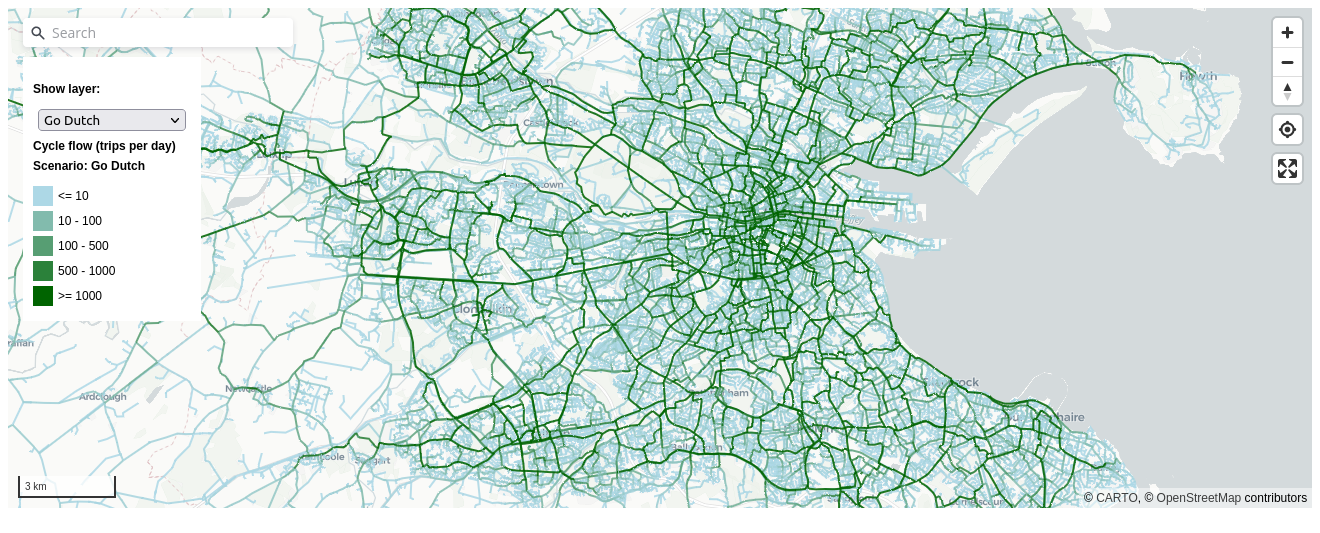
\includegraphics{images/paste-8.png}
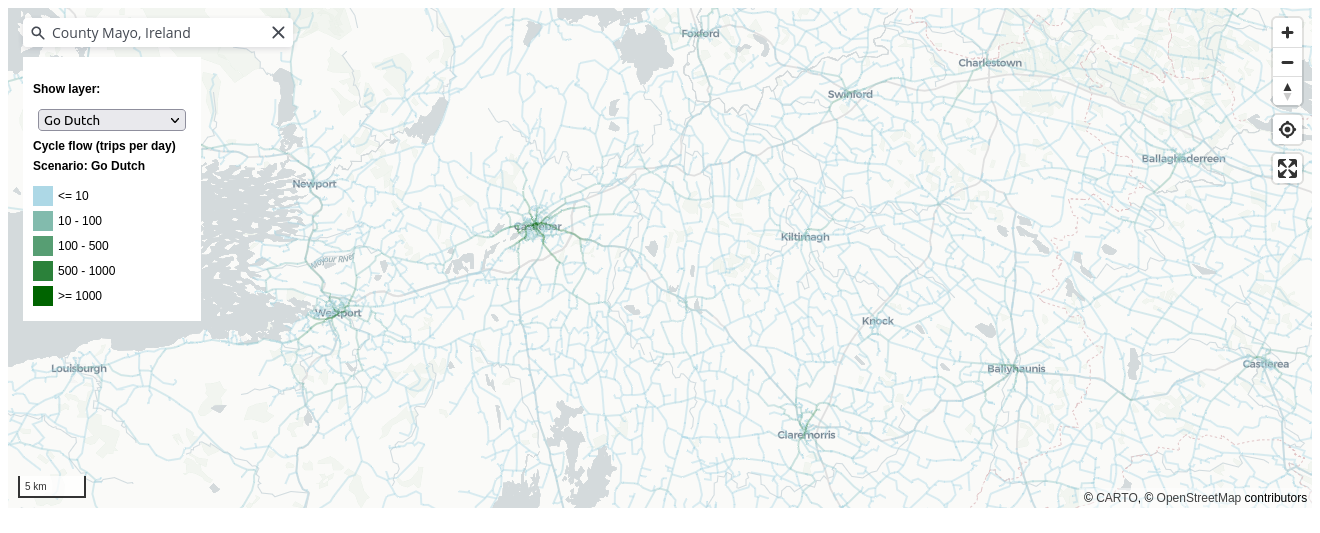
\includegraphics{images/paste-9.png}

}

\caption{\label{fig-dublin}Illustration of the density of route networks
generated by the CRUSE Tool for Dublin City and surroundings (top) and
rural County Mayo on the West coast of Ireland (botton). Source: CRUSE
Tool, publicly available at \href{https://cruse.bike/}{cruse.bike}.}

\end{figure}%

\subsection{Additional trip purposes}\label{sec-trip-purposes}

A limitation of the original PCT was that it only included travel to
work data. This was partially addressed by the inclusion of travel to
school based on data from the Department for Education in England
\citep{goodman2019}. An advantage of the POWSCAR OD data over OD
datasets derived from census surveys in many countries is that it
includes travel to school data. We commissioned a version of POWSCAR
that included a breakdown of the total flows between OD pairs by purpose
and mode, enabling a more realistic estimation of the `Baseline' cycling
network.

However, travel to school and work account for less than half (39\%) of
all trips in Ireland, excluding `returning home' trips, according to the
2022 National Household Travel Survey (NHTS) \citep{national2022}. This
represents a substantial decline in the proportion of trips covered by
POWSCAR data compared with pre-COVID survey results, with 51\% of
non-return trips being for work or education according to the 2017
release of the same report \citep{national2017}. To tackle this issue,
we developed a spatial interaction modeling methodology to estimate the
number of trips between each OD pair for additional trip purposes. The
classification of trip purposes used in the CRUSE Tool was guided mainly
by the trip purpose classification found within the National Household
Travel Survey (NHTS), but with the addition of categories based on the
comprehensive POWSCAR data, and the need to include recreational trips
and multi-stage trips. An overview of the trip purposes used in CRUSE is
presented in Table~\ref{tbl-trip-purposes}.

\begin{longtable}[t]{>{\raggedright\arraybackslash}p{13em}>{\raggedright\arraybackslash}p{15em}>{\raggedright\arraybackslash}p{12em}>{\raggedright\arraybackslash}p{5em}}

\caption{\label{tbl-trip-purposes}Trip purposes used in the CRUSE Tool.}

\tabularnewline

\\
\toprule
Trip purpose & Description & Primary source(s) & Confidence\\
\midrule
\cellcolor{gray!10}{Work (commute)} & \cellcolor{gray!10}{Commuting to/from workplaces} & \cellcolor{gray!10}{Census 2016 POWSCAR Data} & \cellcolor{gray!10}{High confidence - data both origins and destinations for trip purposes}\\
Primary Education & Primary school trips & Census 2016 POWSCAR Data & Dept. of Education Schools database,High confidence - data both origins and destinations for trip purposes\\
\cellcolor{gray!10}{Secondary Education} & \cellcolor{gray!10}{Secondary school trips} & \cellcolor{gray!10}{Census 2016 POWSCAR Data} & \cellcolor{gray!10}{Dept. of Education Schools database,High confidence - data both origins and destinations for trip purposes}\\
Tertiary Education & Tertiary education trips & Census 2016 POWSCAR Data - Geodirectory categories for 'Tertiary Education' and 'Other Education' & High confidence - data both origins and destinations for trip purposes\\
\cellcolor{gray!10}{Social} & \cellcolor{gray!10}{NHTS classification, including trips to/from sports facilities, leisure, and cultural destinations (e.g. restaurants, cinemas, gyms etc.)} & \cellcolor{gray!10}{Trip rates from NHTS} & \cellcolor{gray!10}{Geodirectory businesses classified according to relevant NACE codes,"Medium Confidence - Method should identify clusters of activity for this trip purpose, although individual trips or destinations come with significant uncertainty"}\\
\addlinespace
Shopping & NHTS classification, including trips to/from supermarkets and shops & Trip rates from NHTS & Geodirectory businesses classified according to relevant NACE codes,"Medium Confidence - Method should identify clusters of activity for this trip purpose, although individual trips or destinations come with significant uncertainty"\\
\cellcolor{gray!10}{Personal/other} & \cellcolor{gray!10}{Combination of two NHTS classifications, and includes trips to medical, personal services and others} & \cellcolor{gray!10}{Trip rates from NHTS} & \cellcolor{gray!10}{Geodirectory businesses classified according to relevant NACE codes,"Medium Confidence - Method should identify clusters of activity for this trip purpose, although individual trips or destinations come with significant uncertainty"}\\
Tourism/recreational & Trips by non-resident visitors to/from visitor attractions & Geodirectory listings for accommodation (origins) and destinations (destinations) & Failte Ireland accommodation database, Failte Ireland attraction database,Low confidence - lack of data regarding tourist trip rates\\
\cellcolor{gray!10}{Public Transport} & \cellcolor{gray!10}{Trips to/from public transport} & \cellcolor{gray!10}{NTA Heavy Rail Census} & \cellcolor{gray!10}{NA}\\
\bottomrule

\end{longtable}

Following feedback from stakeholders, we added another, `non-everyday'
trip purpose in an extension phase: cycle tourism. As outlined in the
CRUSE Extension report {[}reference and link to be added on
publication{]}, this involved developing an inter-county spatial
interaction model to estimate the number of trips between each county
for cycle tourism, with trip attractors including campsites and major
international transport hubs.

\subsection{Routing}\label{routing}

Routes in CRUSE are generated by CycleStreets, a not-for profit
transport consultancy and web development company who provide
application programming interfaces (APIs) supplying a range of datasets
for cycle planning and advocacy internationally, including in Ireland.
The CycleStreets routing engine is based on OpenStreetMap (OSM) data,
which is continuously updated by a global community of volunteers.

While CycleStreets offers a free routing API, we commissioned a custom
routing service to enable:

\begin{itemize}
\tightlist
\item
  Calculation of hundreds-of-thousands of routes, which is beyond the
  terms of service of the free API.
\item
  Making changes to the routing profiles, including allowing routing on
  trunk roads, which are sometimes avoided in the default routing
  profiles.
\item
  Control over the version of OSM data being used for the routing,
  allowing regular updates to the route networks as OSM data is updated.
\end{itemize}

The CycleStreets routing engine accounts for hilliness and traffic
signals, based on substantial experience generating cycle routes for
utility and leisure cyclists worldwide. The resulting routes are
designed to indicate the route choices of confident, moderately
confident, and less confident cyclists with three route options provided
for each OD pair as described below. It would be possible to use other
routing engines and custom profiles and cost functions in the future,
for example to simulate the impact of implementing traffic signals which
are optimised for cycling throughput, a feature not currently available
in CycleStreets that could be explored in future work.

We computed three route types for each disaggregated (`jittered') OD
pair: `Fastest', `Balanced' and `Quietest'. As outlined on the
CycleStreets'
\href{https://www.cyclestreets.net/help/journey/howitworks/}{website},
the fastest routes minimize journey time, accounting for traffic lights
and surface type. The `Quietest' route type minimizes busy sections of
road, allowing high `diversion factors' from the fastest route on
quieter but less direct ways (often avoiding roads and interactions with
motor vehicles altogether where possible). The `Balanced' route type is
a compromize between the two, minimising journey time while avoiding the
busiest roads. Allowing users to switch between these three route types
enables them to consider the trade-offs between directness and `cycle
friendliness' when planning new infrastructure, as shown in
Figure~\ref{fig-route-types}. These different network maps are available
on the `Route types' page for each county (see
\href{https://cruse.bike/kildare/route-types}{cruse.bike/kildare/route-types}
for Kildare, for example). In addition to showing the estimated routes
under each scenario, the page also presents summary statistics on the
network:

\begin{itemize}
\item
  On the fastest network, 25\% of the distance cycled occurs in
  non-hostile segments and 7\% in cycle-friendly segments.
\item
  Under the baseline scenario, 52\% of the distance cycled on the
  quietest network occurs in non-hostile segments and 15\% in
  cycle-friendly segments.
\end{itemize}

These statistics can be revealing: in Kildare it suggests that around
half of all cycling activity occurs on network segments that are hostile
(with a high inferred level of traffic stress), even when efforts are
taken to avoid busy segments. For the fastest network, which may be more
realistic for utility cycling, the proportion of cycling on hostile
segments is even higher at 75\%.

\begin{figure}

\begin{minipage}{0.50\linewidth}
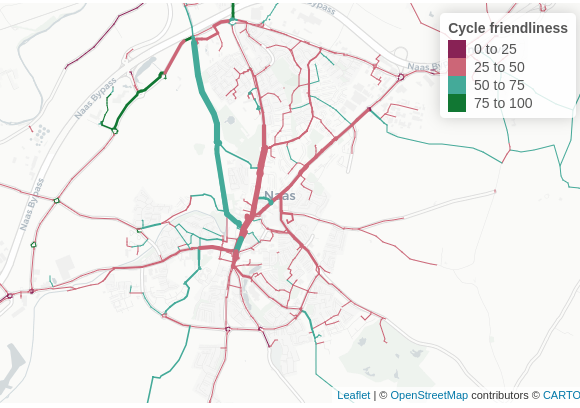
\includegraphics[width=2.60417in,height=\textheight]{images/naas_quietest_godutch.png}\end{minipage}%
%
\begin{minipage}{0.50\linewidth}
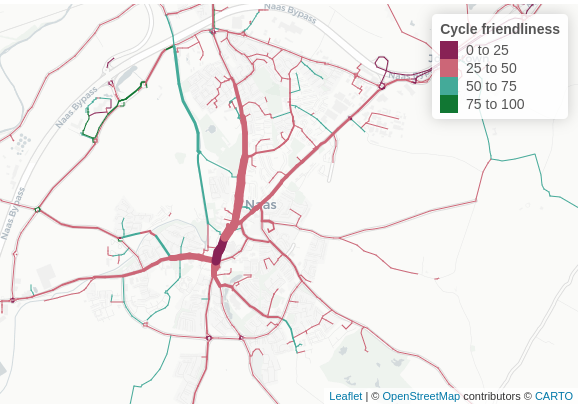
\includegraphics[width=2.60417in,height=\textheight]{images/naas_fastest_godutch.png}\end{minipage}%
\newline
\begin{minipage}{0.50\linewidth}
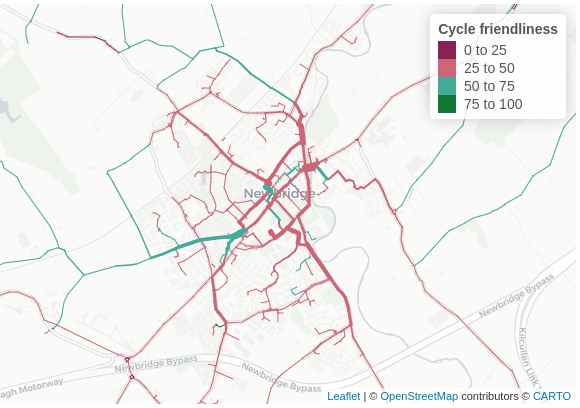
\includegraphics[width=2.60417in,height=\textheight]{images/newbridge_quietest_godutch.png}\end{minipage}%
%
\begin{minipage}{0.50\linewidth}
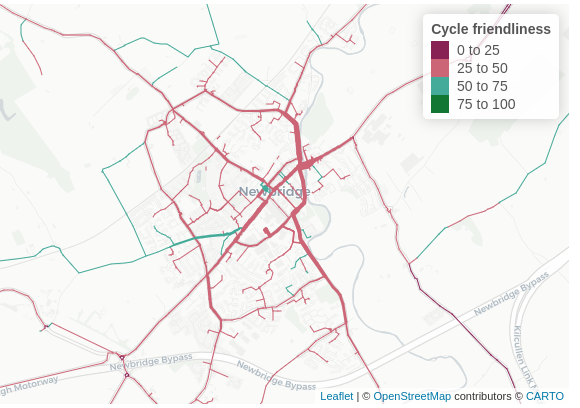
\includegraphics[width=2.60417in,height=\textheight]{images/newbridge_fastest_godutch.png}\end{minipage}%

\caption{\label{fig-route-types}Illustration of the quietest (left) and
fastest (right) route networks for Naas (top) and Newbridge (bottom) in
County Kildare.}

\end{figure}%

\subsection{Scenarios of cycling potential}\label{sec-scenarios}

The datasets outlined above were used to generate estimates of cycling
currently (the `Baseline' scenario) and under four scenarios of cycling
potential: Near Market, Climate Action Plan, Go Dutch, and Ebike. Each
of these scenarios is described below, as illustrated in
Figure~\ref{fig-scenarios}.

\begin{figure}

\centering{

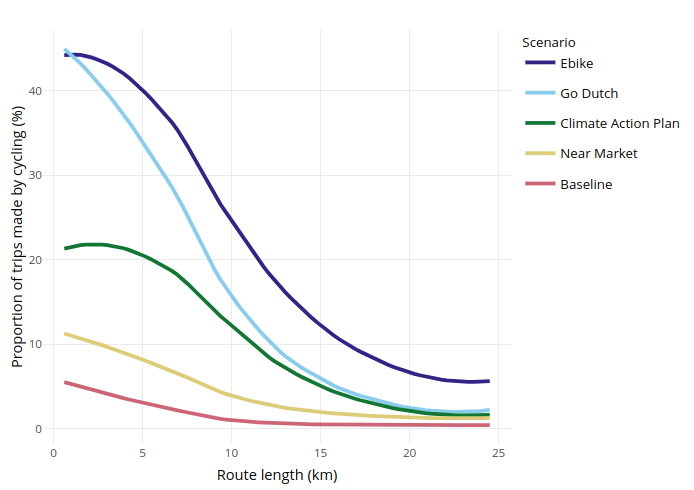
\includegraphics{images/scenarios_kildare.png}

}

\caption{\label{fig-scenarios}Distance-mode share graph for Kildare used
to communicate the different scenarios. Source: county level view for
Kildare in the open access CRUSE Tool at
\url{https://cruse.bike/kildare}.}

\end{figure}%

\subsubsection{Baseline}\label{baseline}

The Baseline scenario approximates current cycling levels. As outlined
in Section~\ref{sec-trip-purposes}, the Baseline scenario includes
travel to work and school, and additional trip purposes. Cycling levels
were taken from the POWSCAR data, which includes the number of people
traveling by each mode between each OD pair.

\subsubsection{Near Market}\label{near-market}

The Near Market scenario approximates the level of cycling that would be
achieved if levels of cycling uptake observed in areas of Ireland with
high levels of cycling according to the 2016 Census were achieved
everywhere, accounting for differences in trip distances and hilliness
levels. The scenario is implemented as follows:

\begin{itemize}
\tightlist
\item
  Calculate distance decay curves for Dublin for the base year (2016,
  using POWSCAR data) by fitting a model to the relevant OD data after
  it has been converted to a route network dataset
\item
  Apply the Near Market model to the hilliness and distance values for
  each county during the build process
\item
  Add the current level of cycling to the Near Market model
\end{itemize}

\subsubsection{Climate Action Plan}\label{climate-action-plan}

The Climate Action Plan scenario models the transport emissions
reductions targeted in the Irish Government's
\href{https://www.gov.ie/en/publication/6223e-climate-action-plan-2021/}{Climate
Action Plan 2021}, which aims for a 51\% cut in overall GHG emissions by
2030 as part of the pathway to net-zero emissions by 2050. For
transport, this includes 500,000 extra walking, cycling and public
transport trips per day by 2030. In terms of car travel, the target is
to ``Increas{[}e{]} the proportion of kilometers driven by passenger
electric cars to between 40 and 45\% by 2030, in addition to a reduction
of 10\% in kilometers driven by the remaining internal combustion engine
cars.'' This equates to a 5.5 to 6\% reduction in total car km driven.

To model this decrease in car km driven, cycling uptake increases in
line with the Go Dutch scenario. However, we only model shift from
driving to cycling. There is no shift from other modes of transport to
cycling.

\subsubsection{Go Dutch}\label{go-dutch}

Under the Go Dutch scenario cycling reaches levels equivalent to those
found in the Netherlands, taking account of the effects of route
hilliness (measured as mean gradient) and route distance. This scenario
uses the same model as the PCT, allowing trips to shift from any other
mode to cycling \citep{lovelace2017}.

\subsubsection{Ebike}\label{ebike}

Also based on the PCT scenario with the same name, the Ebike scenario in
CRUSE takes Go Dutch cycling uptake, and adds onto this the impact of
increased ebike usage, which allows for longer cycle trips. However,
travel to primary and secondary schools still uses Go Dutch uptake,
since no ebike scenario has been developed for school journeys, and
children may be less likely to own ebikes than adults.

\subsection{User interface}\label{sec-ui}

The CRUSE web application is statically hosted, meaning it does not
require a server running software such as the R package `shiny' or
Python packages such as `streamlit' or `flask' in the background
\citep{wickham2021}. This reduces hosting costs and the maintenance
burden of the tool compared with tools such as the PCT, and makes the
map-based interface more responsive, using the recently developed
`MapLibre' JavaScript package and `PMTiles' ``cloud native'' vector tile
format \citep{gonçalves2023}. The default view in landing page is of a
map of Ireland with county level results for the \% trips that could be
made by cycling under the `Go Dutch' scenario, highlighting the intended
use case for strategic cycle network planning and level of ambition. The
key results, route network results, are available within an instant by
zooming in on the map illustrated in Figure~\ref{fig-landing}: beyond a
certain zoom level the network view appears. This differs from the user
interface in tools such as the PCT and BiclaR which force users to click
on a county before the key network results become visible: to get to the
network view in the PCT takes around 10 seconds and multiple clicks,
compared with simply zooming in on the landing page for CRUSE.

Other improvements to the user interface in the national map on the
landing page include a search bar in the top left and clearer legend for
each network visualisation option (users can select any scenario or
quietness or gradient depending on their needs). Following feedback from
user testing, a `geolocate' and `full screen' button were added in the
top right, enabling users to `zoom' to their current location and to
focus on the detailed geographic results, as shown in
Figure~\ref{fig-landing}.

\begin{figure}

\centering{

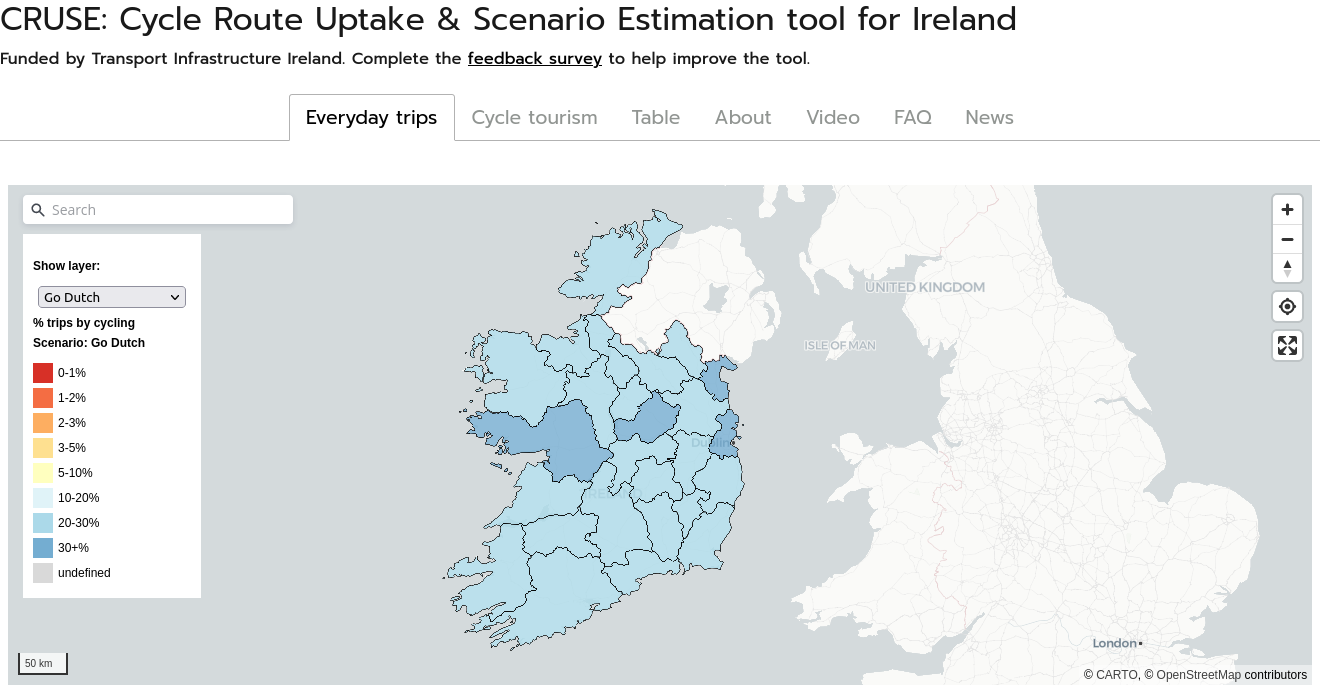
\includegraphics{images/paste-10.png}

}

\caption{\label{fig-landing}Illustration of the landing page of the
CRUSE Tool for Ireland.}

\end{figure}%

Typical intended user stories are illustrated in
Figure~\ref{fig-user-stories}, which shows that the tool is designed to
be used by both professional and non-professional users. For the main
target audience, professional transport planners working at the county
level, the tool provides a range of outputs, including estimates of
cycling potential at the county and network level. The provision of
balanced (the default), quietest and fastest route networks enables
planners to consider the trade-offs between directness and `cycle
friendliness' when planning new infrastructure. The tool also provides
data downloads, enabling estimates of cycling potential on the network
to be visualised and analysed with other tools such as QGIS, Python or
R.

For non-professional users, the tool provides a simple interface to
explore the cycling potential of the network. By providing a single
landing page that is suitable for both professional and non-professional
users (such as an advocate or parent interested in safe routes to
school), the tool aims to facilitate communication between these groups.

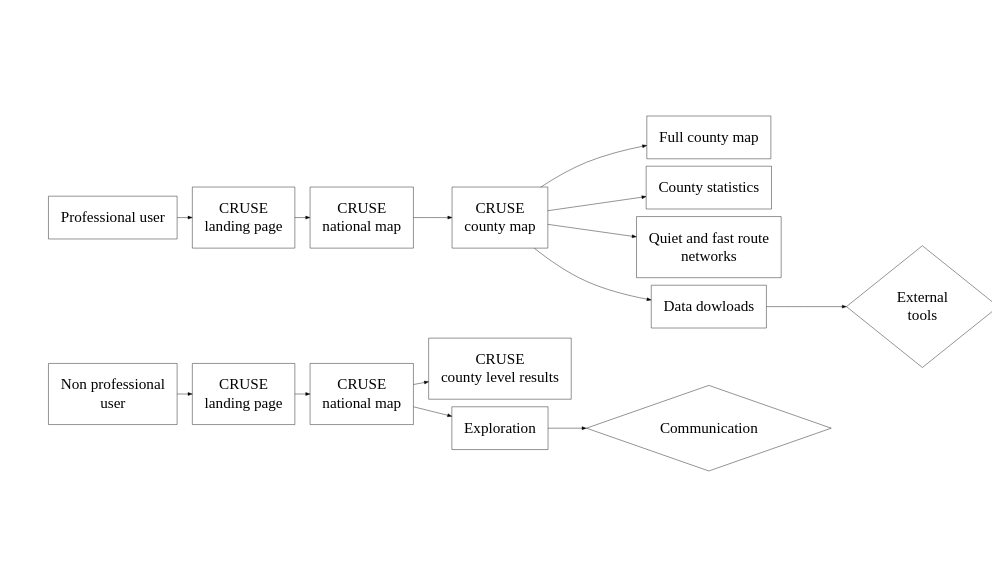
\includegraphics[width=3.31in,height=\textheight]{images/fig5.png}

\begin{figure}

\centering{

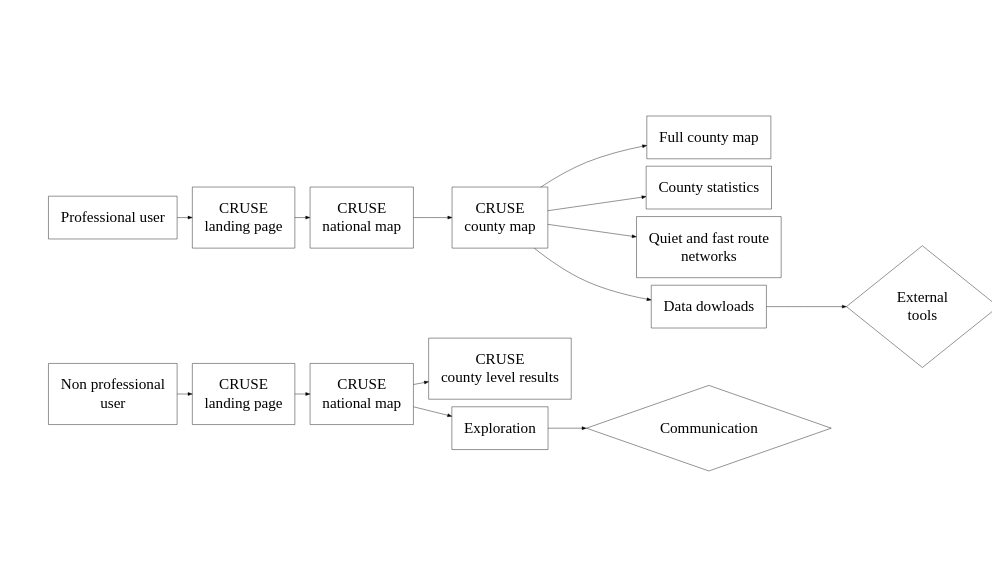
\includegraphics{images/fig5.png}

}

\caption{\label{fig-user-stories}Hypothetical user stories for the CRUSE
Tool illustrating that it can be used in different ways by different
user groups.}

\end{figure}%

\section{Results}\label{sec-results}

The main result of the work presented in this paper is an open access
web application and datasets on current and potential future cycling
levels in Ireland, with evidence provided at county and route segment
levels. Like other national tools presented in Table~\ref{tbl-tools}, a
key feature of the results is that it provides a consistent and
objective baseline for comparing cycling potentials in different areas.

The approach generates estimates of cycling potential on every road in
the country and are therefore too extensive to present in their entirety
in this paper. Through the interactive web application, users can
explore the data to generate the results that are most relevant to their
needs, whether that is finding the cycling potential on a particular
road or finding `weak links' or barriers in the cycle network associated
with a particular school, work place or other destination.

Instead of trying to show such use cases, of which there are many
hundreds, we present a selection of results to illustrate the main
features of the resulting evidence, in Section~\ref{sec-quantiative}. We
also present some qualitative results based on workshops and interviews
with stakeholders in Ireland, in Section~\ref{sec-qualitative}.

\subsection{Selected quantitative results}\label{sec-quantiative}

To illustrate the results in urban areas, we took the top 4 cities in
Ireland by population: Dublin City, Cork, Limerick and Galway (with city
populations of 0.6, 0.2, 0.1 and 0.1 million respectively). In
Figure~\ref{fig-city-results} we present the cycle route networks within
a 3km radius circle centred on each of these cities.

\begin{figure}

\centering{

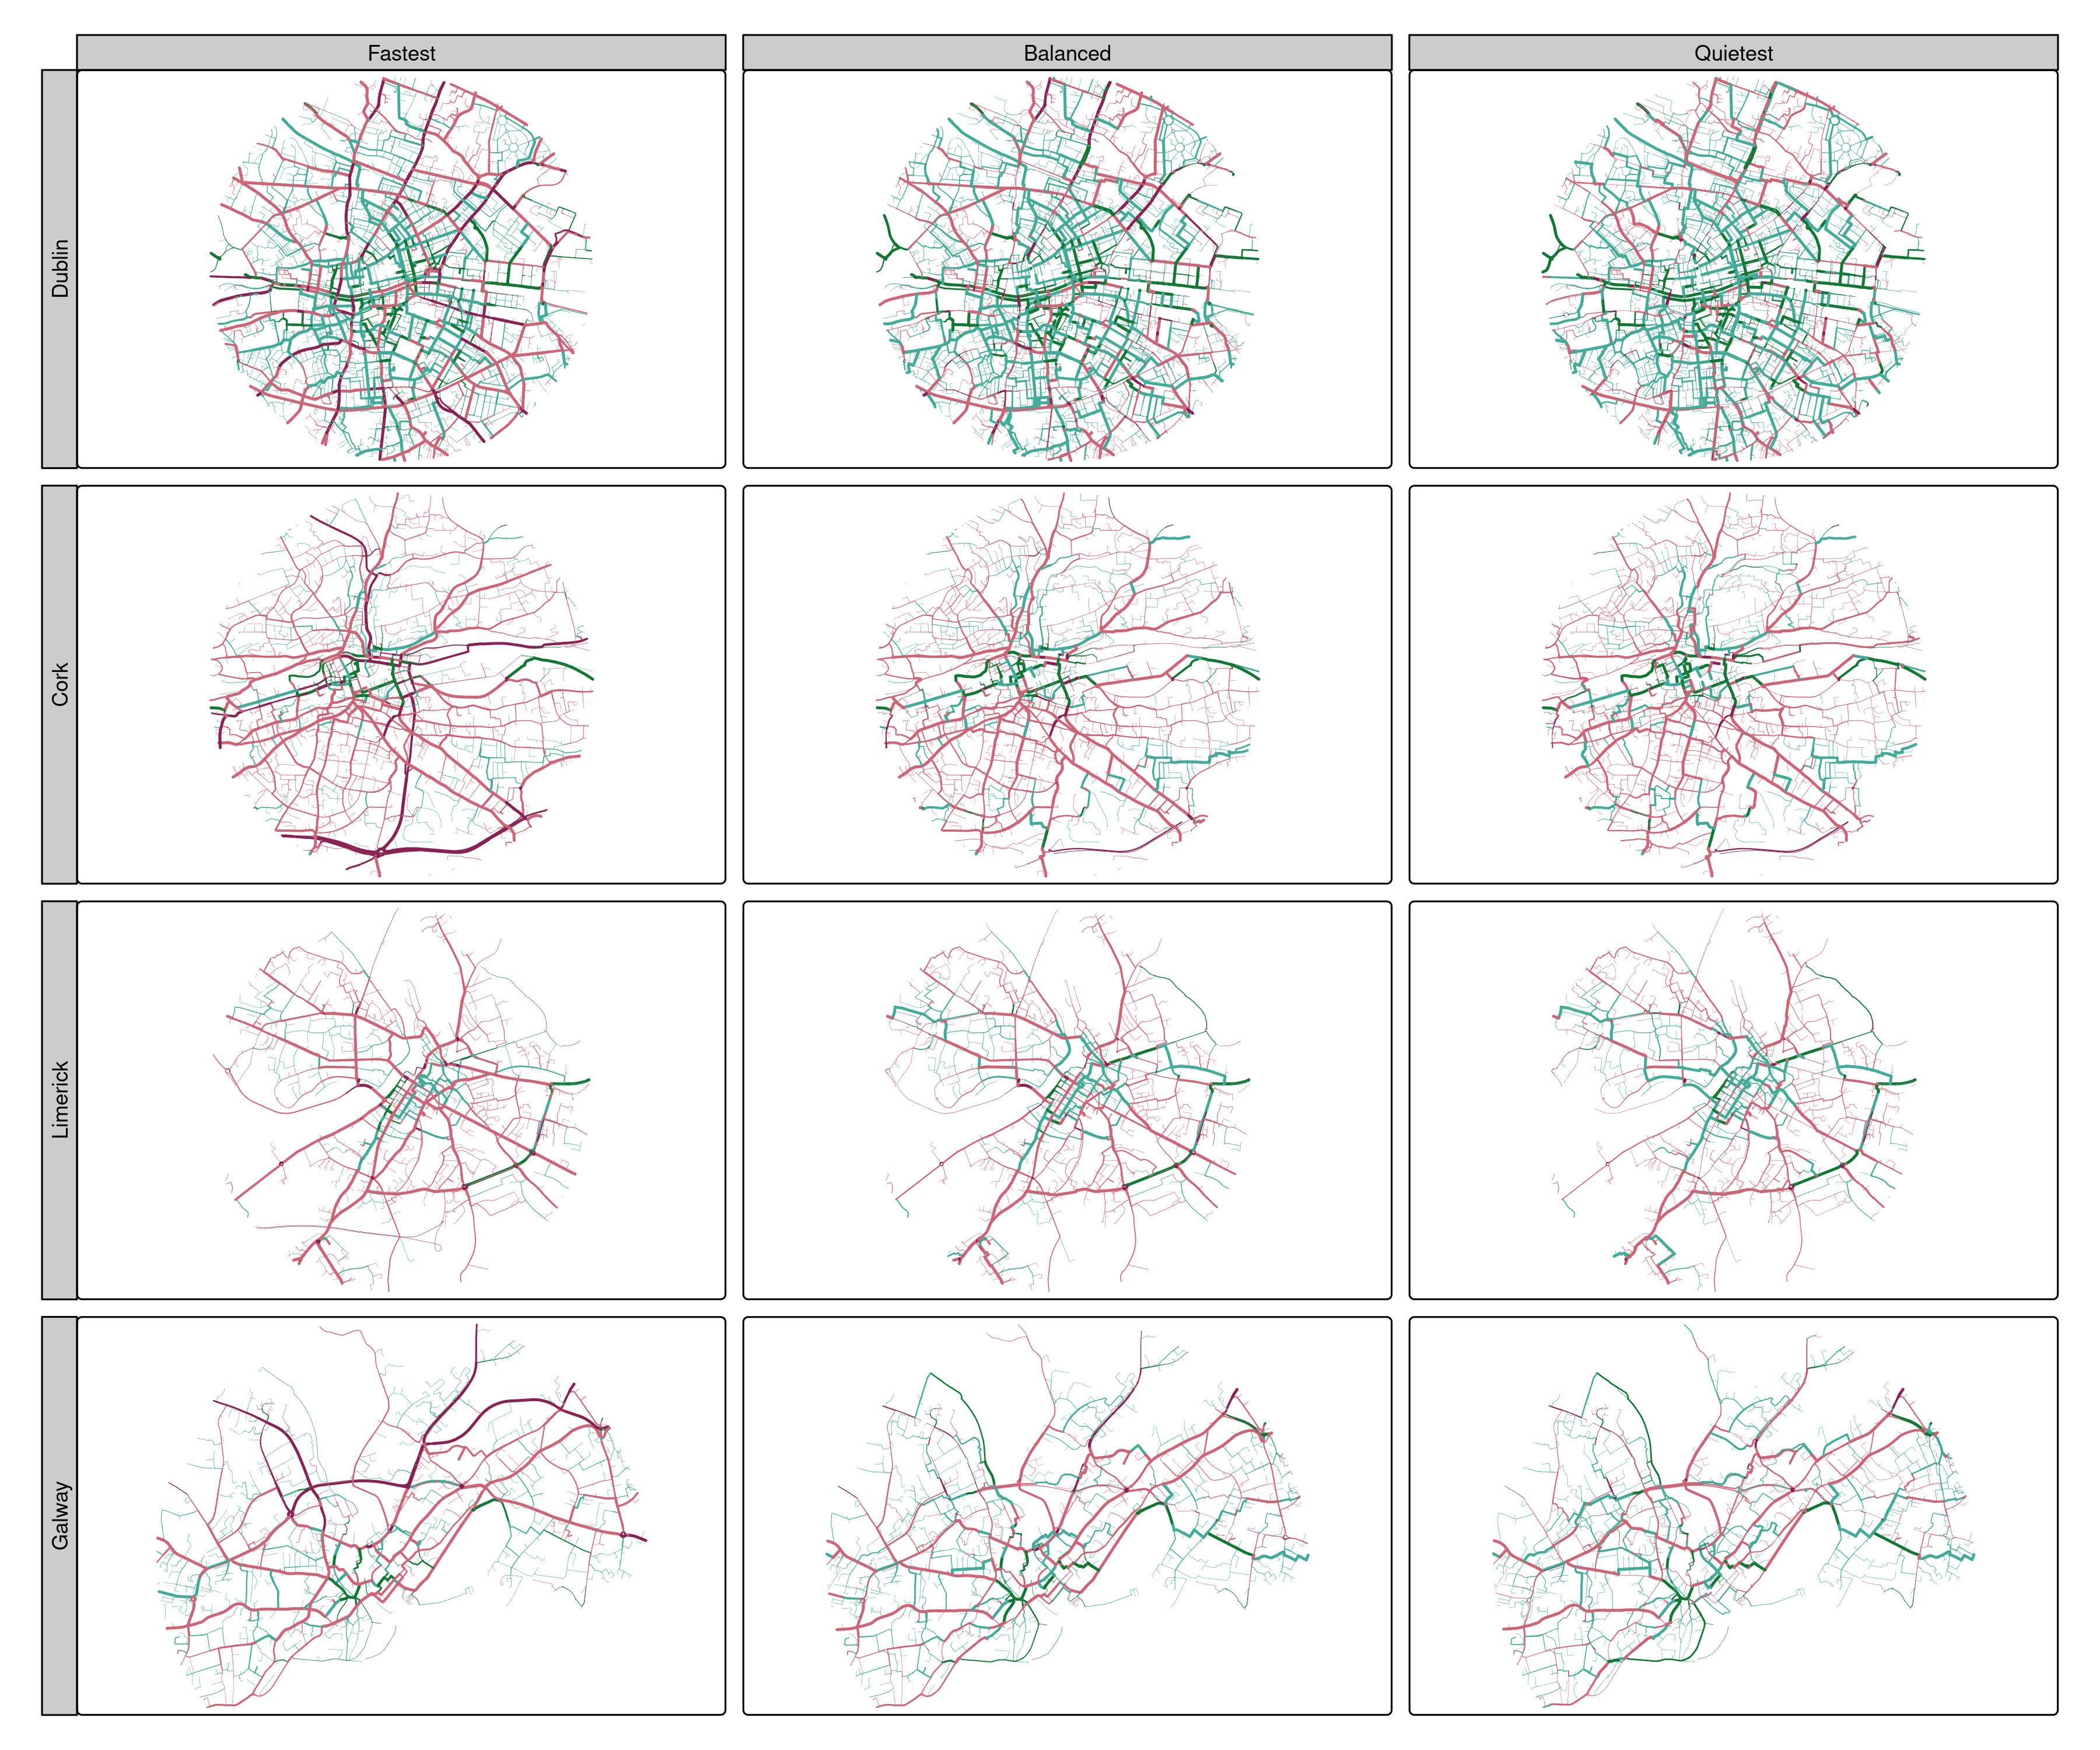
\includegraphics{images/rnet_types.png}

}

\caption{\label{fig-city-results}Fastest, balanced and quietest cycle
networks within 3km circular areas containing the four largest cities in
Ireland. The networks are coloured by cycle friendliness, with greener
segments representing more cycle friendly segments. Widths vary in
proportion to the potential level of cycling under the `Go Dutch'
scenario.}

\end{figure}%

Aside from the widely varying sizes and route networks of each city,
with Dublin having by far the densest network, it is clear from the
visualisation of cycling friendliness that there are many gaps in the
networks. Dublin has had received most investment in cycling
infrastructure and this is apparent from the high proportion of the
route network that is green, even in the fastest route network
representing routes that prioritize speed and directness over comfort
and safety. Dublin also has the highest mode share of cycling of the
four cities, adding to the evidence base showing that investment in
cycling infrastructure is effective in increasing cycling uptake.

Although Dublin City has made progress, there are still many parts of
the fastest route network, and even some parts of the Balanced and
Quietest route networks, that are not cycle friendly and which have high
cycling potential. According to a recent report, 71\% of residents in
the Dublin Metropolitan Area support ``more cycle tracks along roads,
physically separated from traffic and pedestrians'' \citep{walking2021}.
The results for the Dublin area could help prioritise investment in
cycling infrastructure in the city.

\subsection{Stakeholder engagement and feedback}\label{sec-qualitative}

Throughout the project, we undertook a series of workshops and
interviews with stakeholders in Ireland to gather feedback on the
approach and resulting tool. The feedback was generally positive, with
stakeholders commenting on the need for the tool, lack of data on
cycling potential proving a barrier to decision-making and investment,
and the potential for the tool. At an end of project workshop in
December 2023, stakeholders were asked to provide feedback on the tool
and its potential use in practice. Quotes and suggestions from these
workshops, and a subsequent interview with a Senior Transport Planning
using the evidence in their everyday work in Transport Infrastructure
Ireland, and presented in this section (with quotes being attributed to
named individuals where permission has been granted).

Early in the project, we presented the approach to practitioners in
Kildare and Limerick. The feedback from the workshop in Kildare
highlighted the need for the tool for practitioners at the county level,
as highlighted in the following quote:

\begin{quote}
``It's a missing piece of evidence that will help new projects get
built'' (Dónal Hodgins, Senior Engineer, Sustainable Transport \&
Traffic Management, Kildare County Council)
\end{quote}

Practitioners in Kildare County Council found that the evidence
generated \emph{was already valuable} for the development of new cycle
routes, especially when making the case during planning applications.
They emphasized that cycle networks are often fragmented, and the tool
allows them to demonstrate how individual local schemes can contribute
to a larger, interconnected network. An unexpected piece of feedback
from the workshop was the preference for visualizations that directly
compare the fast and quiet routes, as they recognize the importance of
both types of routes. In response to this we provided the `Route types'
page for each county, although this functionality is not available in
the landing page map due to other feedback requesting a simpler
interface. In comparison with another tool for transport planning, CRUSE
was seen by practitioners in Kildare as more user-friendly. They found
the evidence at the route level (unavailable in other tools) crucial for
planning new cycling infrastructure. Overall, the workshop participants
concluded that the approach filled gap in evidence and will greatly
assist in the development of new cycling projects.

During the workshop with practitioners in Limerick, the estimates of
Baseline and Go Dutch potential at the network levels were found to
match well with local knowledge. The tool effectively highlighted the
same sections on the transport network that experienced planners
identified as priorities for investment in cycling, such as the South
Circular Road. Limerick County Council expressed their interest in
utilizing each network layer, particularly the quiet network, to support
new cyclists who lack confidence to share space with motor traffic.
Specific suggestions from the workshop included the suggestion to align
scenarios with national strategy (resulting in the Climate Action Plan
scenario) and to provide data downloads provided as `Shapefiles' for
further analysis (now implemented although the download format is
GeoPackage, an open standard for spatial data).

In a subsequent interview with a practitioner using the evidence
generated by the CRUSE approach in their everyday work, we received the
following feedback. The outputs were found to be a ``useful tool for
getting schemes started; and provides good detail to supplement the
strategic rationale for intervention within Project Outline Documents,
via the cycle friendliness maps and the baseline / near market cyclist
estimates''. As a result, the CRUSE tool ``is ideal for generating a
strategic rationale for estimating demand and building the business case
in the absence of cycle count data; it is also very useful at the
detailed design stage and the CRUSE estimates can (and have been used)
to supplement the economic appraisal of cycling schemes'' (Declan
Keenan, Senior Transport Planner TII working on active travel, personal
communication). Declan also noted a strong alignment in the South Dublin
area between cycle count data, and the outputs of the approach: ``It's
forms a strong representation of what's going on in the areas where TII
have collated some cycling count data, e.g.~in the vicinity of the M50
in the areas of Ballinteer and Sandyford. Some additional network
checking against count data would also be useful, to ensure good
representation across other settlements.'' Where cycling data is
available, the networks align well in terms of network ``shape'' and the
proportion of trips on different parts of the network.

There were two suggestions from Declan which have not yet been
implemented: the provision of data showing POWSCAR and recreational
estimates/data separately, and the need for training on the tool to
ensure that all staff can use it effectively. These, and other potential
improvements, are discussed in the next section.

\section{Discussion}\label{sec-discussion}

The aim of the paper was to describe the design, features and potential
use of the `CRUSE' approach and resulting tool. As outlined in the
previous section, the CRUSE Tool provides evidence on current and
potential future cycling levels across Ireland down to the street level,
with potential assigned to fastest, balanced and quietest route
networks. This provision of multiple scenarios of behavior change
\emph{and} multiple scenarios of investment, for example in cycling
infrastructure next to major roads vs quiet residential streets, is a
key feature of the CRUSE Tool.

\subsection{Uses of the tool in
practice}\label{uses-of-the-tool-in-practice}

As highlighted in a paper on cycling infrastructure preferences based on
a case study of Dublin, both directness and quietness are important
\citep{caulfield2012}:

\begin{quote}
Direct routes with short journey times were found to be the most
important positive variable for existing cyclists and non-cyclists in
determining route choice. This is followed by infrastructure type, the
number of junctions along the route, traffic speed and cyclist volumes.
In terms of infrastructure, regardless of the level of cycling
confidence, routes which have `no facilities' or `bus/cycle lanes' are
the least favoured cycle route types.
\end{quote}

The CRUSE Tool can help both in terms of describing the current
situation, and also prioritise investment in those direct routes with
high cycling potential that lack adequate cycling infrastructure
\citep{caulfield2012}. It will also support reporting for the RISM
Directive on road casualties as part of the road safety management
system.

\subsection{Comparison with other tools and contribution to the
field}\label{comparison-with-other-tools-and-contribution-to-the-field}

While the CRUSE Tool is not the first national and publicly available
tool for cycling planning, it has some key features that make it
relevant for other countries, regions and road authorities tasked with
making their transport systems safe and sustainable:

\begin{itemize}
\tightlist
\item
  The results are \emph{open access} meaning that any stakeholder in the
  planning system can access the evidence. This will help to democratize
  the transport planning process and make wider conversations about
  transport planning more evidence-based and less polarized
  \citep{lovelace2020}, something that is particularly relevant given
  the potentially polarizing nature of pro-cycling interventions
  \citep{wild2017}.
\item
  The results are fully reproducible (code to be released pending
  sign-off by TII's IT team), preventing `cloud lock in' to a
  potentially monopolistic consultancy, and encouraging input from the
  wider open source community \citep{lovelace2021, dhir2017}.
\item
  By covering a wide range of trip purposes --- not just travel to work
  \citep{lovelace2017, heinen2010} and travel to school
  \citep{goodman2019} as covered in previously published research on
  open access national cycle network planning tools --- the results
  capture a higher proportion of cycling potential including key rural
  trips which are often under-represented in models of active travel.
\end{itemize}

As the benefits of strategic planning for cycling become more apparent
\citep{scappini2022}, we expect the demand for tools such as CRUSE to
grow. However, the approach is not without limitations and does not meet
all requirements in Ireland or indeed any country where the methods are
applied.

\subsection{Limitations and future
research}\label{limitations-and-future-research}

The approach has a number of limitations that should be understood by
practitioners, researchers, advocates, policy makers using the tool. As
highlighted in Section~\ref{sec-qualitative}, we were only able to
compare the results with a small number of cycle counters and based on
feedback from workshops. As outlined in the CRUSE extension report
{[}reference to be added on publication{]}, we also undertook validation
against Strava data. However, more data is needed to better understand
the accuracy of the baseline results, especially for the `non-POWSCAR'
purposes. We hope this becomes possible as Ireland's cycle counter
network expands, allowing refinements to the approach (espcially the
spatial interaction model and parameters) to be made. Changes that could
help mitigate this limitation on the user interface side include
providing results with confidence intervals or as categories of cycling
potential, rather than as central estimates, and the visualistion of the
`POWSCAR' network (which is based on Census data) in the web
application.

A limitation associated with the approach is its reliance on
OpenStreetMap (OSM) data. The `cycle friendliness' of a route is based
on the OSM tags and the routes themselves are generated by the
CycleStreets routing engine, which is based on OSM data. During a
conference in Sligo where we presented prelimary results, a stakeholder
with local knowledge pointed out that a quiet route along the canal was
not being followed. In response, manual edits were made to the OSM
network, and the results currently on the website reflect these changes.
However, there are many other potential errors in the OSM data that have
not been corrected. Future work could mitigate this by integrating the
approach more closely with OSM (for example by providing links to enable
one-click edits of OSM when users click on a route segment) or by
setting up a workshop to `crowdsource' corrections to the OSM data.
Furthermore, because there are multiple possible users of the tool with
different starging points, workshops and training events could be
valuable if not essential to ensure that the tool is used effectively.
Such events could bring together stakeholders from advocacy groups,
local authorities, and national governments. The siloed nature of
transport planning means that such diverse stakeholders are rarely the
same room, meaning that a `wide boundary' outcome of the tool could be
to bring these groups together (if workshops based on the tool are
successful).

Another limitation of the approach is that the results are `static',
reducing its ability to support monitoring of growth in cycling,
upgrades of existing cycling infrastructure and dynamic (year-by-year)
exposure information to estimate crash rates. Exposure information is a
key part of the the European RISM Directive, for reporting collision
rates of vulnerable road users by 2024. These factors mean that the tool
can be seen as an open access `leverage point', providing key
information for and supporting ambitious plans in many aspects the
planning system, from network design to post-build monitoring
\citep{lovelace2020}.

\section{Conclusions}\label{sec-conclusions}

The CRUSE Tool is an open access web application for strategic cycle
network planning and prioritization of road safety interventions across
Ireland. Building on previous work, it provides a nationally consistent
evidence base, providing valuable insights to planners and other
stakeholders in the transport planning process, at national and local
levels. Because the results are available at the route segment level,
the tool can be used to identify `weak links' in the cycle network
\citep{vybornova2022}, and to prioritize investment in cycling
infrastructure to maximize health, equality, and other benefits
\citep{mahfouz, woodcock2021}. Furthermore, the provision of the
evidence in a free and publicly available website, hosted at
\href{https://cruse.bike}{cruse.bike}, means that it can be used by
anyone, encouraging wider participation and more evidence-based debate
about transport planning.

A key feature of the project methodologically is its calculation of
current and future potential not only for travel to work and travel to
school, but also for other trip purposes, including recreational trips.
This required the development of spatial interaction models and
estimation of the relative attractiveness of different destinations for
different trip purposes, an area of active research where new
developments could be incorporated into the tool in future
\citep{hasova2022}.

The CRUSE Tool and the underlying research and methods are not without
limitations, suggesting future areas of research, data collection needs,
and policy application. The route network level results have not been
validated to the extent we had planned at the outset of the project. We
compared route network level results with `ground truth' data from cycle
counter datasets across Dublin to test different network types and to
ensure that additional trip types added to work and educational trips
increased the quality of fit under the baseline scenario. However, the
size of the counter network was insufficient to provide an opportunity
for robust evaluation of model performance, suggesting a combined
program of new count data collection and analysis should be a priority
for future work, with findings feeding directly into work to improve the
outputs of the the CRUSE Tool.

More broadly, the tool's outputs are limited to just one mode of active
travel (cycling), ignoring walking and wheeling, including wheelchair
use and a range of wheeled devices such as scooters, bike trailers and
e-cargo bikes that can be used to escort children to school. Sustainable
transport policies should plan for walking, wheeling and cycling, and
there are many co-benefits of broadly defined active travel
interventions that benefit all active modes, such as measures to reduce
heavy motor traffic speeds and volumes in areas and along corridors with
high active travel potential. This raises the question of whether other
active modes should be incorporated into the results using the OD-based
approach outlined in this paper, or whether different modeling
approaches are needed to properly capture the shorter distance trips
typically made by walking \citep{cooper2018}. Furthermore, the estimates
of cycling presented in the CRUSE Tool omit multi-modal trips including
public transport, and omit trip chaining, due to the need to capture a
large portion of cycling potential within the resource constraints of
the project.

The CRUSE Tool is already used in practice to support more ambitious and
data-driven planning for safe cycling routes in multiple counties across
Ireland. We hope that the underlying approach, and the publicly
available evidence provided in the CRUSE Tool itself, provide a basis
for future reproducible research, open source software development into
strategic cycle network planning tools in Ireland and other countries.
Active travel represents a win-win-win for physical activity,
environment, and local economic opportunities. In combination with
broader sustainable mobility measures and policies to reduce motor
traffic speeds and volumes, tools such as CRUSE can support the fast and
fair decarbonisation of transport systems worldwide.

\section{List of abbreviations}\label{list-of-abbreviations}

APIs: Application Programming Interfaces

CSO: Central Statistics Office

CRUSE: Cycle Route Uptake and Scenario Estimation

ED: Electoral Division

GHG: Greehouse Gas

GTFS: General Transit Feed Specification

KSI: Killed and Seriously Injured

NRA: National Road Authority

NRN: National Road Network

OD: Origin-Destination, typically referring to origin-destination data
which contains information on the number of people traveling between
each pair of zones

OSM: Open Street Map

PCT: Propensity to Cycle Tool

POWSCAR: Place of Work, School or College Census of Anonymized Records

TII: Transport Infrastructure Ireland

\section{Declarations}\label{declarations}

\subsection*{Availability of data and
material}\label{availability-of-data-and-material}
\addcontentsline{toc}{subsection}{Availability of data and material}

Data was obtained from the Central Statistics Office (CSO) and Transport
Infrastructure Ireland (TII) under license and cannot be shared
publicly. The code used to generate the results presented in this paper
is fully reproducible and available at {[}to be added post review.{]}

\subsection*{Funding}\label{funding}
\addcontentsline{toc}{subsection}{Funding}

This work was funded by Transport Infrastructure Ireland (TII).

\subsection*{Acknowledgements}\label{acknowledgements}
\addcontentsline{toc}{subsection}{Acknowledgements}

{[}To be added post review.{]}


  \bibliography{references.bib}


\end{document}
